\section{Theoretical Analysis} \label{section:theo}


\par In this section, a theoretical analysis of the circuit shown in section \ref{introduction} was conducted. 

\subsection{Description and Important Mathematical considerations}


We also computed the low cutoff frequency and the high cut off frequency in octave. The central frequency was also calculated, using the following expression:

\begin{equation}
\omega_{0}= \sqrt{\omega_{L} * \omega_{H}}
\end{equation}



\subsection{Final Results}
All the important results obtained are shown in the tables and in the figure bellow. 

\begin{figure}[h] \centering
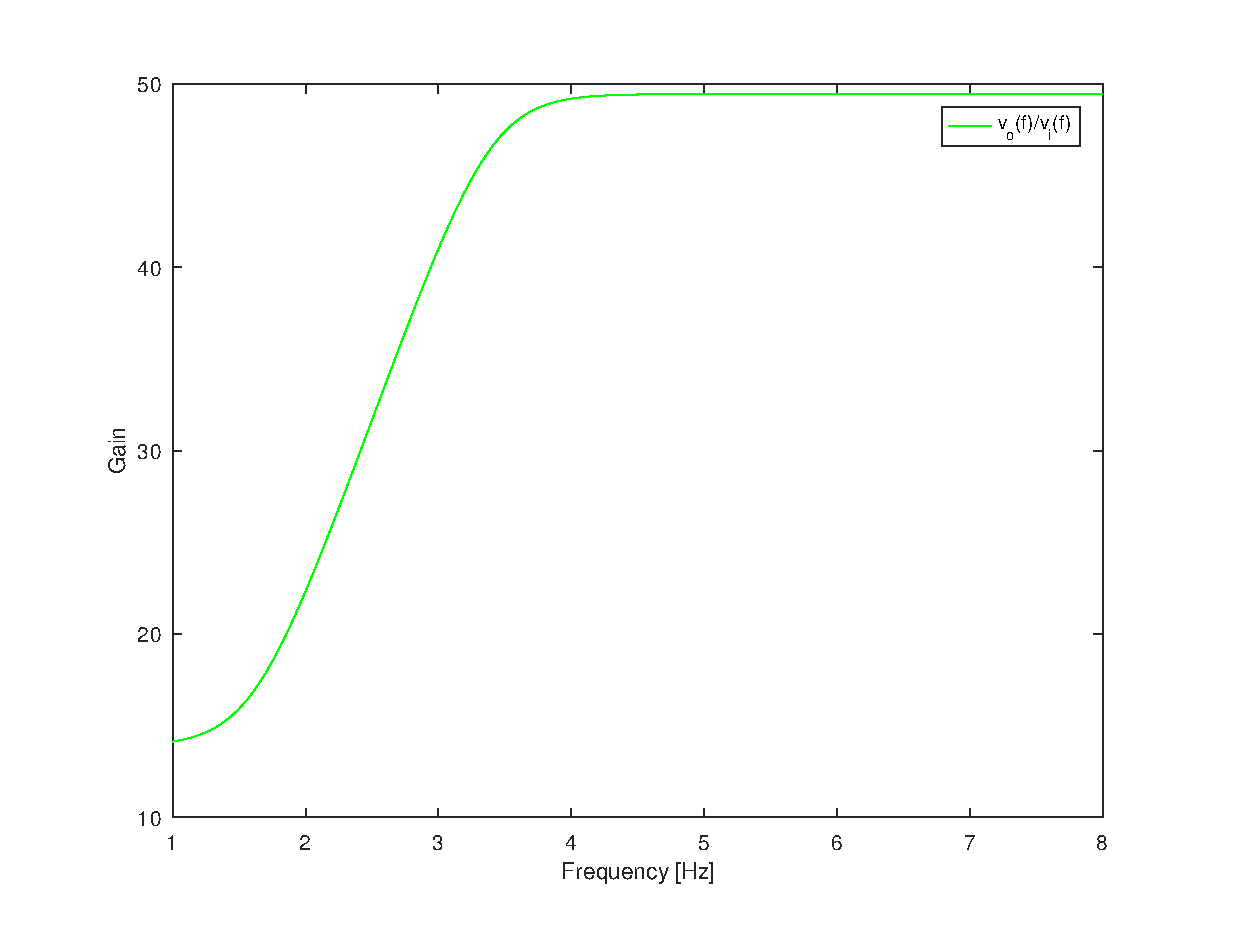
\includegraphics[width=0.65\linewidth]{theo.eps}
\caption{Voltage Gain of the circuit. Octave}
\label{sh}
\end{figure}




\begin{table}[ht]
  \centering
  \begin{tabular}{|l|r|}
    \hline    
    {\bf Name} & {\bf Value} \\ \hline
    \input{../mat/impedances_tab}
  \end{tabular}
  \caption{Input and output Impedences}
  \label{tab:2}
\end{table}



\begin{table}[ht]
  \centering
  \begin{tabular}{|l|r|}
    \hline    
    {\bf Name} & {\bf Value} \\ \hline
    \input{../mat/band_pass_freq_tab}
  \end{tabular}
  \caption{Low cut-off frequency, High cut-off frequency, Central Frequency.}
\end{table}



\begin{table}[ht]
  \centering
  \begin{tabular}{|l|r|}
    \hline    
    {\bf Name} & {\bf Value} \\ \hline
    \input{../mat/wo_freq_gain_tab}
  \end{tabular}
  \caption{Central Frequency(Hz) and Respective Gain(dB).}
\end{table}


\begin{table}[ht]
  \centering
  \begin{tabular}{|l|r|}
    \hline    
    {\bf Name} & {\bf Value} \\ \hline
    \input{../mat/Cost_Merit_tab}
  \end{tabular}
  \caption{Cost and Merit.}
\end{table}











